\documentclass[11pt,a4paper]{article}

% Build: latexmk -pdf -interaction=nonstopmode -halt-on-error
%        jupyterlab_student_guide.tex
% All illustrations are drawn in LaTeX; no external assets are required.
\usepackage[T1]{fontenc}
\usepackage[utf8]{inputenc}
\usepackage[default]{sourcesanspro}
\usepackage{inconsolata}
\usepackage{amsmath,amssymb}
\usepackage[a4paper,margin=19mm,top=20mm,bottom=20mm,headheight=15pt]{geometry}
\usepackage{xcolor}
\usepackage{microtype}
\usepackage{graphicx}
\usepackage{tikz}
\usetikzlibrary{arrows.meta,positioning}
\usepackage[most]{tcolorbox}
\usepackage{listings}
\usepackage{upquote}
\usepackage{enumitem}
\usepackage{tabularx,booktabs,array}
\usepackage{fancyhdr,lastpage}
\usepackage{hyperref}
\input{glyphtounicode}
\pdfgentounicode=1

\definecolor{ink}{HTML}{183247}
\definecolor{muted}{HTML}{526471}
\definecolor{accent}{HTML}{007D86}
\definecolor{pale}{HTML}{EAF5F4}
\definecolor{papergray}{HTML}{F3F5F7}
\definecolor{linegray}{HTML}{D5DEE4}
\definecolor{orange}{HTML}{BD5917}

\hypersetup{colorlinks=true,urlcolor=accent,linkcolor=accent,
  pdftitle={Getting started with JupyterLab},
  pdfsubject={Student practice guide using NumPy, SciPy and Matplotlib},
  pdfkeywords={JupyterLab, JupyterLite, Python, NumPy, SciPy, Matplotlib}}
\urlstyle{same}
\setlength{\parindent}{0pt}
\setlength{\parskip}{6pt}
\setlength{\emergencystretch}{2em}
\renewcommand{\arraystretch}{1.18}
\setlist[itemize]{leftmargin=1.35em,itemsep=3pt,topsep=3pt}
\setlist[enumerate]{leftmargin=1.55em,itemsep=4pt,topsep=3pt}
\pagestyle{fancy}
\fancyhf{}
\fancyhead[L]{\small\color{muted}JUPYTERLAB \; / \; STUDENT PRACTICE GUIDE}
\fancyfoot[L]{\small\color{muted}Practice in your browser}
\fancyfoot[R]{\small\color{muted}\thepage\ / \pageref*{LastPage}}
\renewcommand{\headrulewidth}{0pt}
\renewcommand{\footrulewidth}{0pt}

\newcommand{\key}[1]{\texttt{#1}}
\newcommand{\code}[1]{\texttt{#1}}
\newcommand{\ui}[1]{\textbf{#1}}
\newcommand{\pagetitle}[3]{%
  \phantomsection\addcontentsline{toc}{section}{#1. #2}%
  {\small\bfseries\color{accent}#1\quad #3\par}
  \vspace{2mm}{\LARGE\bfseries\color{ink}#2\par}\vspace{2mm}}
\newcommand{\sub}[1]{\par\vspace{2mm}{\large\bfseries\color{ink}#1\par}\vspace{0.5mm}}
\newcommand{\cell}[1]{\par\vspace{1mm}{\small\bfseries\color{accent}#1\par}\vspace{-1mm}}
\newtcolorbox{note}[1]{enhanced,colback=pale,colframe=pale,
  borderline west={2pt}{0pt}{accent},boxrule=0pt,arc=1mm,
  left=3mm,right=3mm,top=2mm,bottom=2mm,
  title={#1},coltitle=ink,fonttitle=\bfseries,
  colbacktitle=pale,attach title to upper={\par\smallskip}}
\lstdefinestyle{python}{language=Python,basicstyle=\ttfamily\small,
  keywordstyle=\color{accent}\bfseries,commentstyle=\color{muted},
  stringstyle=\color{orange},backgroundcolor=\color{papergray},
  frame=single,rulecolor=\color{linegray},framerule=0.35pt,
  framesep=3mm,xleftmargin=3mm,xrightmargin=3mm,
  aboveskip=6pt,belowskip=6pt,showstringspaces=false,
  keepspaces=true,columns=fullflexible,upquote=true,
  breaklines=true,tabsize=4}
\lstset{style=python}

\begin{document}
\color{ink}

% ----------------------------------------------------------------------
\pagetitle{01}{Getting started with JupyterLab}{OPEN YOUR FIRST NOTEBOOK}
{\large A practical introduction with NumPy, SciPy and Matplotlib\par}

\textbf{Allow about 35--45 minutes.} You only need a computer with a keyboard,
an up-to-date web browser, an internet connection and basic Python knowledge.
You will create a notebook, run calculations, draw a figure and keep a copy
of your work.

\begin{note}{Where to practise}
Open the official demo: \href{https://jupyter.org/try-jupyter/lab/}{\textbf{jupyter.org/try-jupyter/lab/}}.
No account or local installation is needed. This demo uses JupyterLite,
which runs Python inside your browser.\par
\textbf{This is a practice environment.} Your actual exams take place on the
course's own server. Follow the instructor's directions for exam access
and submission.
\end{note}

\sub{Create a notebook}
\begin{enumerate}
  \item Let the page finish loading. You may see an introductory notebook;
        you can leave it open or close its tab.
  \item Click the \ui{+} above the file list on the left to open the
        \ui{Launcher}. Under \ui{Notebook}, choose a \ui{Python} kernel.
        Its label may include \ui{XPython} or \ui{Pyodide}; do not choose
        a different programming language.
  \item Right-click the new file in the file list, choose \ui{Rename},
        and call it \code{jupyter\_practice.ipynb}. Keep the
        \code{.ipynb} extension: it identifies a Jupyter notebook.
  \item Click in the empty cell, type the code below, then press
        \key{Shift+Enter}. Wait for the first imports to finish.
\end{enumerate}

\cell{Code cell 1 --- import the libraries}
% verify: imports
\begin{lstlisting}
import numpy as np
import scipy
from scipy.integrate import trapezoid
import matplotlib
import matplotlib.pyplot as plt

print("NumPy:", np.__version__)
print("SciPy:", scipy.__version__)
print("Matplotlib:", matplotlib.__version__)
\end{lstlisting}

Three version numbers should appear below the cell. Their exact values
may change. The demo's Python environment includes all three libraries;
you do not need to install them for this guide.

\textbf{First checkpoint:} you have a named notebook and a cell that runs.
If you see an import error, check that the notebook is using a Python
kernel and try restarting it (page~3).

\vfill
{\small\color{muted}\textbf{Route through the guide:}
interface and cells (2) \;\textbullet\; kernel and execution order (3)
\;\textbullet\; calculations (4) \;\textbullet\; plots (5)
\;\textbullet\; upload and download (6) \;\textbullet\; files and recovery (7)
\;\textbullet\; independent practice (8).}

\newpage
% ----------------------------------------------------------------------
\pagetitle{02}{Find your way around}{THE INTERFACE AND ITS CELLS}
The notebook is a sequence of \textbf{cells}. Select a cell to work on it;
its output appears immediately below it.

\begin{center}
% notebook-figure: interface
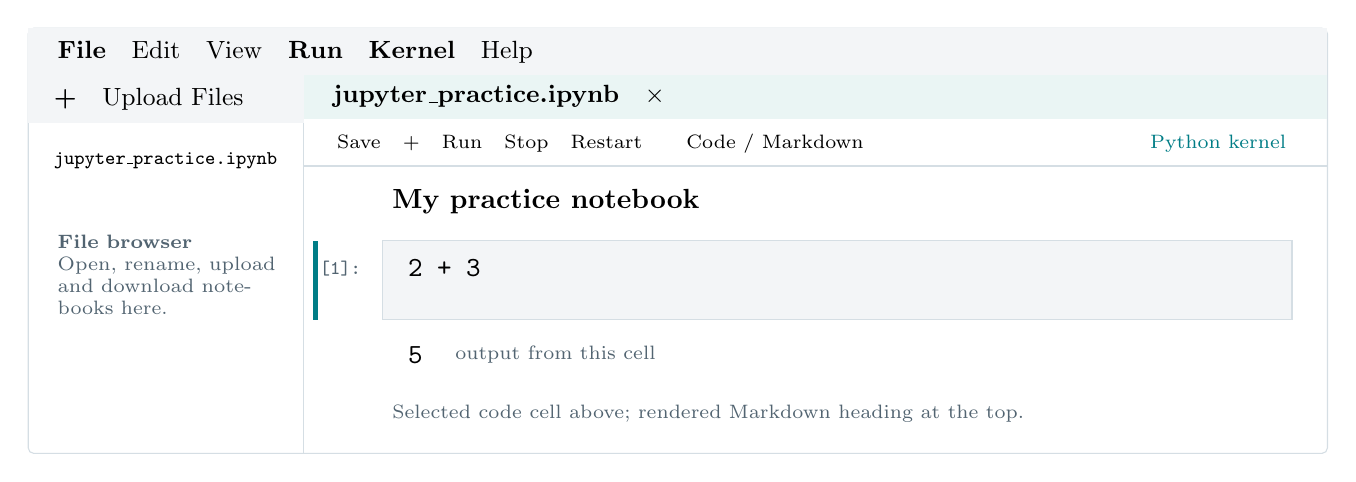
\begin{tikzpicture}[x=1cm,y=1cm,font=\small]
  \filldraw[fill=white,draw=linegray,rounded corners=2pt] (0,0) rectangle (16.5,5.4);
  \fill[papergray] (0,4.8) rectangle (16.5,5.4);
  \node[anchor=west] at (.25,5.1)
       {\textbf{File}\quad Edit\quad View\quad\textbf{Run}\quad\textbf{Kernel}\quad Help};
  \draw[linegray] (3.5,0) -- (3.5,4.8);
  \fill[papergray] (0,4.2) rectangle (3.5,4.8);
  \node[anchor=west] at (.2,4.5) {\textbf{+}\quad Upload Files};
  \node[anchor=north west,font=\ttfamily\scriptsize] at (.2,3.95)
       {jupyter\_practice.ipynb};
  \node[anchor=north west,text width=2.85cm,font=\scriptsize\color{muted}]
       at (.25,2.9) {\textbf{File browser}\\Open, rename, upload and download notebooks here.};
  \fill[pale] (3.5,4.25) rectangle (16.5,4.8);
  \node[anchor=west] at (3.75,4.53) {\textbf{jupyter\_practice.ipynb}\quad $\times$};
  \node[anchor=west,font=\scriptsize] at (3.8,3.94)
       {Save\quad +\quad Run\quad Stop\quad Restart\qquad Code / Markdown};
  \node[anchor=east,font=\scriptsize\color{accent}] at (16.1,3.94) {Python kernel};
  \draw[linegray] (3.5,3.65) -- (16.5,3.65);
  \node[anchor=west,font=\bfseries] at (4.5,3.2) {My practice notebook};
  \draw[accent,line width=2pt] (3.65,1.7) -- (3.65,2.7);
  \filldraw[fill=papergray,draw=linegray] (4.5,1.7) rectangle (16.05,2.7);
  \node[anchor=east,font=\ttfamily\scriptsize\color{muted}] at (4.35,2.35) {[1]:};
  \node[anchor=west,font=\ttfamily] at (4.7,2.35) {2 + 3};
  \node[anchor=west,font=\ttfamily] at (4.7,1.25) {5};
  \node[anchor=west,font=\scriptsize\color{muted}] at (5.3,1.25) {output from this cell};
  \node[anchor=west,font=\scriptsize\color{muted}] at (4.5,.5)
       {Selected code cell above; rendered Markdown heading at the top.};
\end{tikzpicture}\par
{\small\color{muted}Simplified interface map. Icons, labels and spacing may vary.}
\end{center}

\sub{Use the two cell types}
\textbf{Code} cells execute Python. Add a cell below your imports using
the notebook toolbar's \ui{+} button. Type \code{2 + 3} and run it with
\key{Shift+Enter}; the output is \code{5}.

\textbf{Markdown} cells contain explanations, headings and equations.
Add another cell, change \ui{Code} to \ui{Markdown} using the toolbar
drop-down, then type this:
\begin{lstlisting}[language={},keywordstyle={},stringstyle={}]
# My practice notebook
I am using **NumPy**, **SciPy** and **Matplotlib**.
An equation: $y = \sin(x)$.
\end{lstlisting}
Run it with \key{Shift+Enter} to format the text. Double-click the
formatted text to edit it again. Markdown is explanatory text; it does
not define Python variables.

\sub{Switch between typing and arranging cells}
\textbf{Edit mode:} click inside a cell or press \key{Enter} to type.
\textbf{Command mode:} press \key{Esc} to act on the whole cell.
In command mode, \key{B} inserts a cell below, \key{A} inserts one above,
\key{M} changes it to Markdown and \key{Y} changes it to Code.
These letters are not shortcuts while you are typing inside a cell.

\begin{note}{Try it}
Create a temporary cell, enter \code{10 * 2} and run it. Delete that
cell using its context menu's \ui{Delete Cells} action, then use
\ui{Edit > Undo Cell Operation} to restore it. You can also press
\key{Esc}, then \key{Z}, to undo a cell deletion.
\end{note}

\newpage
% ----------------------------------------------------------------------
\pagetitle{03}{Understand what is running}{THE KERNEL AND EXECUTION ORDER}
The \textbf{notebook} stores your cells and any saved outputs. The
\textbf{kernel} runs the code and holds variables in memory. All code
cells in one notebook normally share that memory.

\sub{Run this small experiment}
Add the following three code cells \emph{below} the cells already in
your practice notebook. Run them in order.

\cell{Cell A}
% verify: state-a
\begin{lstlisting}
a = 10
\end{lstlisting}
\cell{Cell B}
% verify: state-b
\begin{lstlisting}
b = a + 1
\end{lstlisting}
\cell{Cell C}
% verify: state-c
\begin{lstlisting}
print(a, b)
\end{lstlisting}
The output is \code{10 11}. Now change Cell A to \code{a = 20} and run
\textbf{only A and C}. You get \code{20 11}: Cell B has not run again,
so \code{b} still contains its earlier value. Run B, then C, to obtain
\code{20 21}.

\begin{note}{Editing a cell does not execute it}
After changing a cell, run it again \emph{and} rerun any later cells that
depend on it. Existing outputs do not update automatically. The numbers
beside code cells show execution order, which can differ from page order.
\end{note}

\sub{Read the execution indicator}
\begin{tabularx}{\linewidth}{@{}>{\ttfamily}p{19mm}X@{}}
\toprule
{[\ ]} & The cell has no execution count yet.\\
{[*]} & The cell is executing or waiting for the kernel.\\
{[7]} & This was the kernel's seventh numbered execution.\\
\bottomrule
\end{tabularx}

An assignment such as \code{a = 10} normally produces no output.
Use \code{print(a)} or put \code{a} on the last line to display it.

\sub{Restart and check the whole notebook}
Open \ui{Kernel > Restart Kernel and Run All Cells\ldots} and confirm.
The kernel forgets its variables, then executes the notebook from the
top. If the command is labelled differently, use \ui{Restart Kernel}
followed by \ui{Run > Run All Cells}. This checks that all the code you
need is actually present and in the right order.

Restarting alone does not delete your cell text. Saved outputs can
remain visible even though their variables no longer exist in memory.
If a calculation takes too long, try \ui{Kernel > Interrupt Kernel}.
If the browser kernel does not respond, try restarting it; avoid running
the same slow cell repeatedly.

\newpage
% ----------------------------------------------------------------------
\pagetitle{04}{Calculate with NumPy and SciPy}{ONE CELL AT A TIME}
Continue in the same notebook. Keep the imports from page~1 at the top.
Each block below goes into a \textbf{separate Code cell}. Copy the code
only; do not copy the expected output.

\sub{NumPy: work with a whole array}
% verify: array
\begin{lstlisting}
values = np.array([1.0, 2.0, 3.0, 4.0])
print(values**2)
print(values.mean())
\end{lstlisting}
Expected output:
\begin{lstlisting}[language={}]
[ 1.  4.  9. 16.]
2.5
\end{lstlisting}
\code{values**2} squares every element. Python uses \code{**} for
powers. Array indexing starts at zero: \code{values[0]} is \code{1.0}.

\sub{Build sample points for a sine curve}
% verify: samples
\begin{lstlisting}
x = np.linspace(0, np.pi, 201)
y = np.sin(x)
print(x.shape, y.shape)
\end{lstlisting}
Expected output: \code{(201,) (201,)}. The arrays contain 201 matching
sample points, including both endpoints. NumPy's trigonometric functions
use radians. The variables \code{x} and \code{y} remain available to
the following cells.

\sub{SciPy: approximate the area under the curve}
% verify: integral
\begin{lstlisting}
area = trapezoid(y, x=x)
print(f"Integral estimate: {area:.6f}")
print(f"Absolute error: {abs(area - 2):.6f}")
\end{lstlisting}
Expected output:
\begin{lstlisting}[language={}]
Integral estimate: 1.999959
Absolute error: 0.000041
\end{lstlisting}
Here \code{trapezoid} is the function imported from \code{scipy.integrate}.
It approximates an integral from sampled data. The exact comparison is
\[
  \int_0^\pi \sin(x)\,\mathrm{d}x = 2.
\]
The formatting \code{:.6f} displays six digits after the decimal point;
it does not round the value stored in \code{area}.

\begin{note}{Make a change and follow its effects}
Replace \code{201} by \code{21} in the sampling cell. Rerun that cell
and the integration cell. Compare the error, then restore \code{201}
and rerun both. Merely changing the number in the editor is not enough.
\end{note}

\newpage
% ----------------------------------------------------------------------
\pagetitle{05}{Draw and explain a figure}{MATPLOTLIB AND MARKDOWN}
Add a Code cell after the integration cell. It uses \code{x} and
\code{y} from page~4, so run their definition first.

% verify: plot
\begin{lstlisting}
fig, ax = plt.subplots(figsize=(6, 3))
ax.plot(x, y, label="sin(x)")
ax.fill_between(x, y, alpha=0.15)
ax.set_xlabel("x (radians)")
ax.set_ylabel("y")
ax.set_title("Area under a sine curve")
ax.grid(True, alpha=0.3)
ax.legend()
fig.tight_layout()
plt.show()
\end{lstlisting}

Run the cell. A figure like this should appear \textbf{below the code},
inside the notebook.

\begin{center}
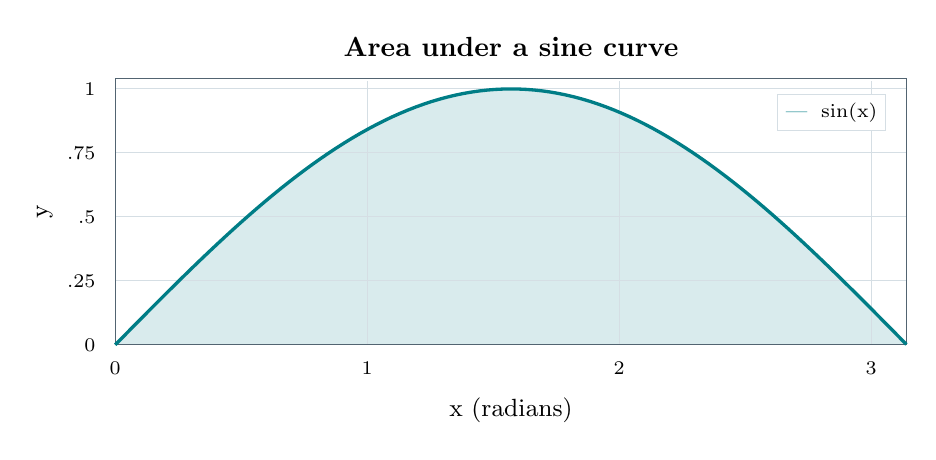
\begin{tikzpicture}[x=3.2cm,y=3.25cm,font=\small]
  \fill[accent!15] (0,0) -- plot[domain=0:pi,samples=101]
      (\x,{sin(\x r)}) -- (pi,0) -- cycle;
  \foreach \y in {0,.25,.5,.75,1} {
    \draw[linegray,thin] (0,\y) -- (pi,\y);
    \node[anchor=east,font=\scriptsize] at (-.04,\y) {\y};
  }
  \foreach \x/\t in {0/0,1/1,2/2,3/3} {
    \draw[linegray,thin] (\x,0) -- (\x,1.03);
    \node[anchor=north,font=\scriptsize] at (\x,-.03) {\t};
  }
  \draw[muted] (0,0) rectangle (pi,1.04);
  \draw[accent,line width=1.2pt] plot[domain=0:pi,samples=101]
       (\x,{sin(\x r)});
  \node[anchor=south,font=\bfseries] at (pi/2,1.09) {Area under a sine curve};
  \node[anchor=north] at (pi/2,-.17) {x (radians)};
  \node[rotate=90] at (-.28,.52) {y};
  \node[anchor=north east,fill=white,draw=linegray,inner sep=3pt,
        font=\scriptsize] at (3.06,.98) {\textcolor{accent}{---}\; sin(x)};
\end{tikzpicture}
\end{center}

\sub{Explain your result in a Markdown cell}
Add a cell below the plot, change its type to \ui{Markdown}, enter the
following, then press \key{Shift+Enter}.
\begin{lstlisting}[language={},keywordstyle={},stringstyle={}]
## Numerical integration
The estimated area is approximately **2**.
The exact result is $\int_0^{\pi} \sin(x)\,dx = 2$.
\end{lstlisting}

\sub{Practise updating a figure}
Change the plot title and rerun the plotting cell. Then change the
sample count on page~4, rerun that sampling cell, the integration cell
and the plotting cell. Each run creates a fresh figure because the
cell begins with \code{plt.subplots()}.

\textbf{Checkpoint:} you can combine executable code, numerical output,
a labelled figure and a written explanation in one notebook.

\newpage
% ----------------------------------------------------------------------
\pagetitle{06}{Upload and download files}{MOVE NOTEBOOKS, DATA AND FIGURES}
\textbf{Upload} copies a file from your computer into JupyterLab.
\textbf{Download} copies a file from JupyterLab to your computer.
These actions work for notebooks (\code{.ipynb}), data and figures.

\sub{Upload an existing notebook}
\begin{enumerate}[itemsep=2pt,parsep=0pt,topsep=2pt]
  \item Open the folder containing the \code{.ipynb} file in your
        computer's file manager (File Explorer or Finder). Place this
        window beside your browser.
  \item In JupyterLab's left sidebar, open the \textbf{file browser}
        and select the destination folder.
  \item Click and hold the local file, drag it onto the \textbf{file list
        in JupyterLab's left sidebar}, then release. You can select
        several files to upload together.
  \item Wait for its name to appear, then double-click it to open.
        Select a Python kernel if asked.
\end{enumerate}
Or click \ui{Upload Files} (the upward arrow above the file list)
and choose the notebook.

\noindent\begin{minipage}{\linewidth}\centering
% notebook-figure: upload
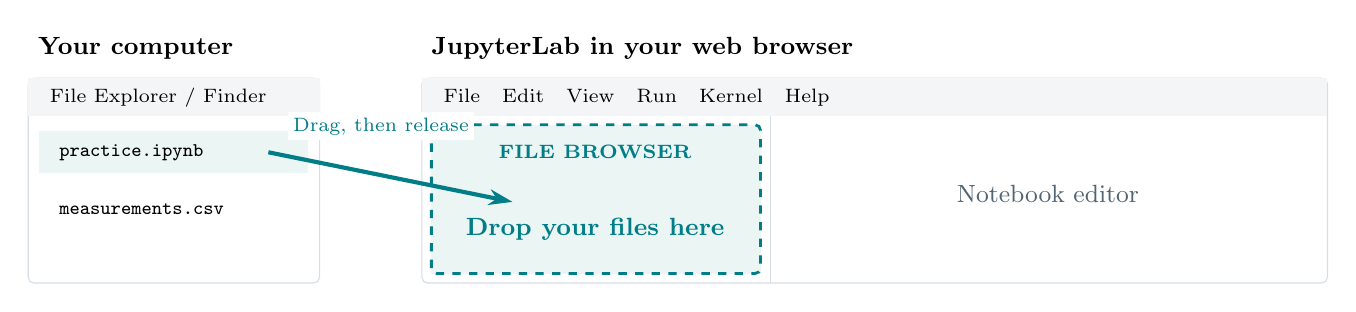
\begin{tikzpicture}[x=1cm,y=1cm,font=\small]
  \node[anchor=south west,font=\bfseries\small] at (0,2.72) {Your computer};
  \filldraw[fill=white,draw=linegray,rounded corners=2pt]
       (0,0) rectangle (3.7,2.6);
  \fill[papergray] (0,2.12) rectangle (3.7,2.6);
  \node[anchor=west,font=\scriptsize] at (.15,2.36) {File Explorer / Finder};
  \fill[pale] (.14,1.4) rectangle (3.55,1.93);
  \node[anchor=west,font=\ttfamily\scriptsize] at (.27,1.66) {practice.ipynb};
  \node[anchor=west,font=\ttfamily\scriptsize] at (.27,.94) {measurements.csv};
  \node[anchor=south west,font=\bfseries\small] at (5,2.72)
       {JupyterLab in your web browser};
  \filldraw[fill=white,draw=linegray,rounded corners=2pt]
       (5,0) rectangle (16.5,2.6);
  \fill[papergray] (5,2.12) rectangle (16.5,2.6);
  \node[anchor=west,font=\scriptsize] at (5.15,2.36)
       {File\quad Edit\quad View\quad Run\quad Kernel\quad Help};
  \fill[pale] (5.12,.12) rectangle (9.3,2.01);
  \draw[accent,dashed,line width=1pt,rounded corners=2pt]
       (5.12,.12) rectangle (9.3,2.01);
  \node[anchor=north,font=\scriptsize\bfseries\color{accent}] at (7.2,1.88)
       {FILE BROWSER};
  \node[align=center,font=\bfseries\small\color{accent}] at (7.2,.68)
       {Drop your files here};
  \draw[linegray] (9.43,0) -- (9.43,2.12);
  \node[font=\small\color{muted}] at (12.95,1.13) {Notebook editor};
  \draw[-{Stealth[length=3mm,width=2mm]},accent,line width=1.5pt]
       (3.05,1.66) -- (6.15,1.03);
  \node[fill=white,inner sep=2pt,font=\scriptsize\color{accent}]
       at (4.48,1.99) {Drag, then release};
\end{tikzpicture}\par
{\small\color{muted}Simplified diagram: the shaded file list on the left is the upload target.}
\end{minipage}\par

\sub{Download your notebook}
\begin{enumerate}[itemsep=2pt,parsep=0pt,topsep=2pt]
  \item Save your latest notebook edits: use the Save button or
        \key{Ctrl+S} (\key{Cmd+S} on macOS).
  \item In the left file browser, \textbf{right-click your notebook's
        \code{.ipynb} filename and choose Download}.
  \item Find the \code{.ipynb} copy in Downloads, or the folder chosen
        in your browser. Upload it again to reopen and continue later.
\end{enumerate}
Download data and figures the same way (examples on page~7).

\sub{Upload and read a data file}
Upload the supplied \code{measurements.csv} to the \textbf{same folder as
your notebook}, using the button or drag and drop. In a new Code cell, run:
% verify: load-data
\begin{lstlisting}
import numpy as np
data = np.loadtxt("measurements.csv", delimiter=",", skiprows=1)
print(data.shape)
\end{lstlisting}
Expected output: \code{(5, 2)} --- five data rows and two columns.
\code{np.loadtxt} reads the data; \code{skiprows=1} skips the header.

\begin{note}{Save and download are different actions}
Save writes to browser storage; Download keeps a copy on your computer.
Download your work before leaving: clearing site data, using private
browsing or switching browsers can make the demo's stored files unavailable.
\end{note}

\newpage
% ----------------------------------------------------------------------
\pagetitle{07}{Keep your results and recover from errors}{FILES AND TROUBLESHOOTING}

\sub{Create files to download}
After running the sine-curve cells on pages~4--5, run this Code cell.
It saves the figure and a CSV containing the plotted data.
% verify: export-files
\begin{lstlisting}
fig.savefig("sine_curve.png", dpi=150, bbox_inches="tight")
np.savetxt("sine_data.csv", np.column_stack((x, y)),
           delimiter=",", header="x,y", comments="")
\end{lstlisting}
The files are written to the kernel's current folder, normally the
notebook's folder in this demo. Refresh the file browser if needed,
then right-click each filename and choose \ui{Download}. Saving a file
from Python does not automatically download it to your computer.

\sub{Reopen a saved notebook}
Save and download your practice notebook. Rename the copy to
\code{reopened.ipynb} on your computer, then upload and open it as
described on page~6. Upload \code{measurements.csv} to the same folder
too, before restarting the kernel and running all cells.

\begin{note}{Keep the input files with your notebook}
A notebook contains code and saved outputs, not live Python variables or
copies of the data files its code reads. A relative filename such as
\code{measurements.csv} is resolved from the kernel's current folder;
Python in the demo cannot read your computer's Downloads folder directly.
\end{note}

\sub{When something goes wrong}
\begin{tabularx}{\linewidth}{@{}>{\raggedright\arraybackslash}p{40mm}
                                   >{\raggedright\arraybackslash}X@{}}
\toprule
\textbf{What you see} & \textbf{What to try}\\
\midrule
\code{FileNotFoundError} & Check the exact filename and its extension,
and upload the file to the notebook's folder. Use \code{import os}, then
\code{print(os.getcwd())} and \code{print(os.listdir())} to inspect the
kernel's current folder and files.\\[3pt]
\code{NameError} & Read the variable name in the last line of the error.
Check its spelling and run the cell that defines it. For \code{np},
\code{plt} or \code{trapezoid}, rerun the imports.\\[3pt]
\code{SyntaxError} or \code{IndentationError} & Check the highlighted line,
brackets, quotes, colons and indentation. Fix the code and rerun the cell.\\[3pt]
\code{TypeError} or \code{ValueError} & Read the last line of the traceback.
Check the function's inputs and the shapes of your arrays.\\[3pt]
A cell stays at \code{[*]} & Allow time for initial loading. For a stuck
calculation, try \ui{Kernel > Interrupt Kernel}, then restart if necessary.\\[3pt]
Old or unexpected output & Rerun the cells that define the data and then
the cells that use it. If uncertain, restart and run all.\\[3pt]
An import fails & Confirm that a Python kernel is selected, then restart
and rerun the imports. If it still fails, ask the instructor.\\
\bottomrule
\end{tabularx}

\textbf{Getting help:} type \code{np.sin?} in a Code cell and run it to
request function help. You can also use \code{help(np.sin)}. Press
\key{Tab} after part of a name, such as \code{np.lin}, to request
completion; \key{Shift+Tab} inside a function call requests its tooltip.

\newpage
% ----------------------------------------------------------------------
\pagetitle{08}{Try it on your own}{FINAL PRACTICE AND QUICK REFERENCE}
\textbf{Allow about 10 minutes for this final check.} Create a new Python
notebook named \code{final\_practice.ipynb}. Refer to earlier pages
when you need them.

\begin{enumerate}
  \item Add a Markdown heading and one sentence explaining the task.
  \item Import NumPy, Matplotlib and \code{trapezoid} from SciPy.
  \item Create 101 equally spaced points from 0 to 1 and calculate
        \(y=x^2\). Remember: Python writes the square as \code{x**2}.
  \item Approximate the integral with \code{trapezoid(y, x=x)}. Display
        the estimate and its absolute error relative to \(1/3\).
  \item Plot the curve with a title and labels for both axes.
  \item Restart the kernel and run all cells. Resolve any errors, save
        the notebook and download it to your computer.
\end{enumerate}

\textbf{Check your result:} the integral estimate is approximately
\code{0.333350}; the absolute error is approximately \code{0.000016667}.
The curve rises from \((0,0)\) to \((1,1)\).

\sub{Useful keyboard shortcuts}
Click inside the notebook before using these shortcuts. In the table,
``\key{Esc}, then'' means press and release \key{Esc} first.

\begin{tabularx}{\linewidth}{@{}p{49mm}X@{}}
\toprule
\textbf{Keys} & \textbf{Action}\\
\midrule
\key{Shift+Enter} & Run the selected cell and select the next cell.\\
\key{Ctrl+Enter} & Run the selected cell and stay on it.\\
\key{Esc}, then \key{A} / \key{B} & Insert a cell above / below.\\
\key{Esc}, then \key{M} / \key{Y} & Change the cell to Markdown / Code.\\
\key{Enter} / \key{Esc} & Enter edit mode / command mode.\\
\key{Esc}, then \key{Z} & Undo the most recent cell operation.\\
\key{Ctrl+S} & Save the active notebook.\\
\bottomrule
\end{tabularx}
{\small On macOS, use \key{Cmd} in place of \key{Ctrl}. Menu commands
provide an alternative if a browser or keyboard intercepts a shortcut.}

For graded work, keep provided cells and metadata, and follow the required
names, arguments and return values. Use the course server and the
instructor's submission procedure for exams.

\vfill
{\footnotesize\color{muted}
\textbf{Official references}\quad
\href{https://jupyterlab.readthedocs.io/en/stable/user/interface.html}{JupyterLab interface}
\;\textbullet\;
\href{https://jupyterlab.readthedocs.io/en/stable/user/notebook.html}{Notebooks}
\;\textbullet\;
\href{https://jupyterlab.readthedocs.io/en/stable/user/files.html}{Files}
\;\textbullet\;
\href{https://jupyterlab.readthedocs.io/en/stable/user/commands.html}{Commands}
\;\textbullet\;
\href{https://jupyterlite.readthedocs.io/en/stable/quickstart/using.html}{JupyterLite}\par
\href{https://numpy.org/doc/stable/user/absolute_beginners.html}{NumPy basics}
\;\textbullet\;
\href{https://docs.scipy.org/doc/scipy/reference/generated/scipy.integrate.trapezoid.html}{SciPy trapezoid}
\;\textbullet\;
\href{https://matplotlib.org/stable/users/explain/quick_start.html}{Matplotlib quick start}
\;\textbullet\;
\href{https://github.com/jupyter/try-jupyter/blob/main/environment-python.yml}{Demo's Python packages}\par
\href{https://numpy.org/doc/stable/reference/generated/numpy.loadtxt.html}{Reading CSV data}
\;\textbullet\;
\href{https://jupyterlite.readthedocs.io/en/stable/howto/content/python.html}{Files in browser kernels}.\par
Prepared October 2026. Menu labels and package versions may change.}

\end{document}
